\documentclass[english]{article}

\usepackage{graphicx}

\usepackage{grffile}

\usepackage[T1]{fontenc}

\usepackage{babel}

\usepackage{float}

\usepackage{tabu}

\usepackage{ragged2e}

\usepackage{textcomp}

\usepackage{amstext}

\usepackage{pdfpages}



\graphicspath{{/}}



\begin{document}

\title{Testing Of Team Broadsword Access User }

\author{Team longsword Access }

\date{May 2017}

\maketitle



	\begin{figure}

		
\includegraphics[width=\linewidth]{up_logo.png}

	\end{figure}

	

	\begin{center}

	 \line(1,0){370}

	\\[0.2cm]

    	{\scshape\Large Testing phase  \par}

	\vspace{0.1cm}

	\line(1,0){370}

	\\[0.8cm]

	

	 {\scshape\Large Team List \par}

	\vspace{0.9cm}

	

	\begin{tabu} to \textwidth { X[l] X[l]}

		\hline

		\textbf{Surname, First Name  }	& \textbf{Student Number}	\\ \hline \hline

		   &	\\ \hline

		  &	\\ \hline

		  &	\\ \hline

	    	 &	\\ \hline

		van der Westhuizen Idrian&15078729\\ \hline Merissa Joubert &15062440	\\ \hline

		\hline

	\end{tabu}

	

	\end{center}



	\pagenumbering{gobble}

	\newpage

	\tableofcontents



	\pagenumbering{arabic}

	\newpage



\section{Users}










\section{Notifications}



\section{Data}



\section{GIS}

\section{Service Contracts}

1.	Service GIS request\\
	a.	Get XYZ coordinates of a named location\\
2.	Add GIS information\\
	a.	Add a location with coordinates to the system\\
3.	Modify GIS information\\
4.	Remove GIS information\\
5.	Update GIS Map\\
6.	Modify GIS Map\\




\subsection{Service GIS request}

\begin{figure}[ht!]

\hspace*{-2.5cm} 

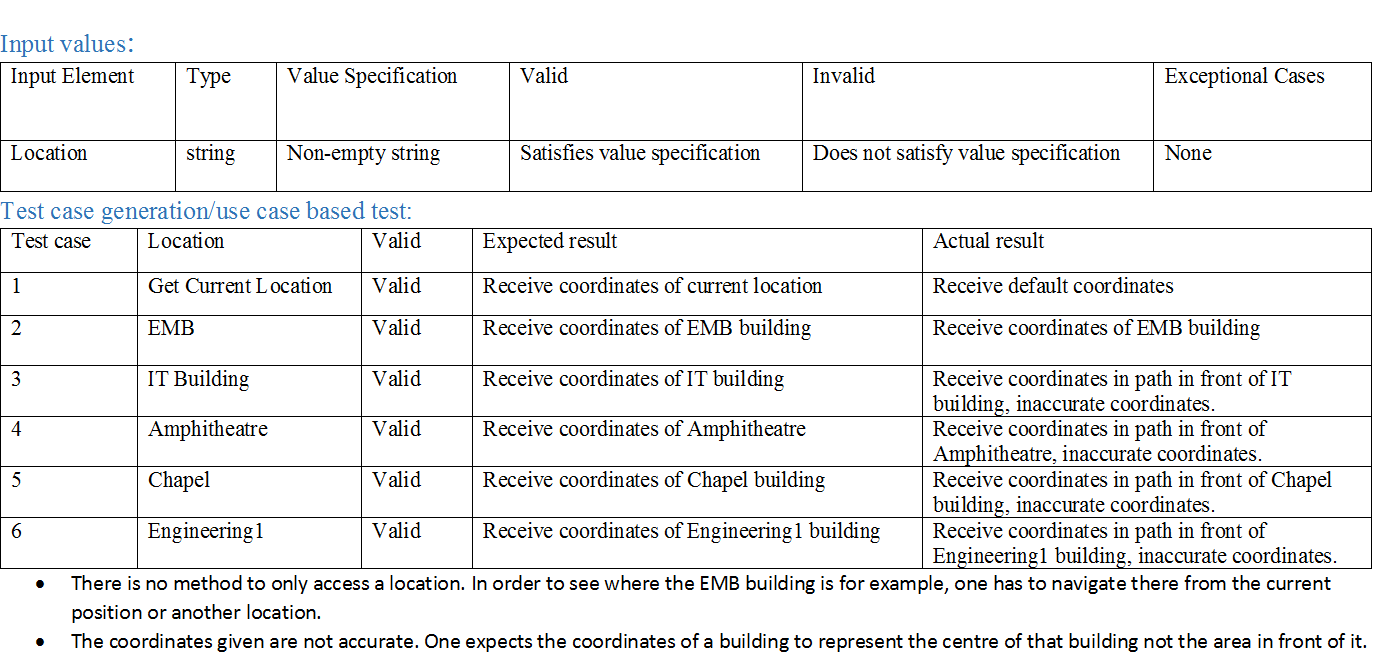
\includegraphics[width=180mm]{ServiceGISReq.png}

\end{figure}


\subsection{Add GIS information}

\begin{figure}[ht!]

\hspace*{-2.5cm} 

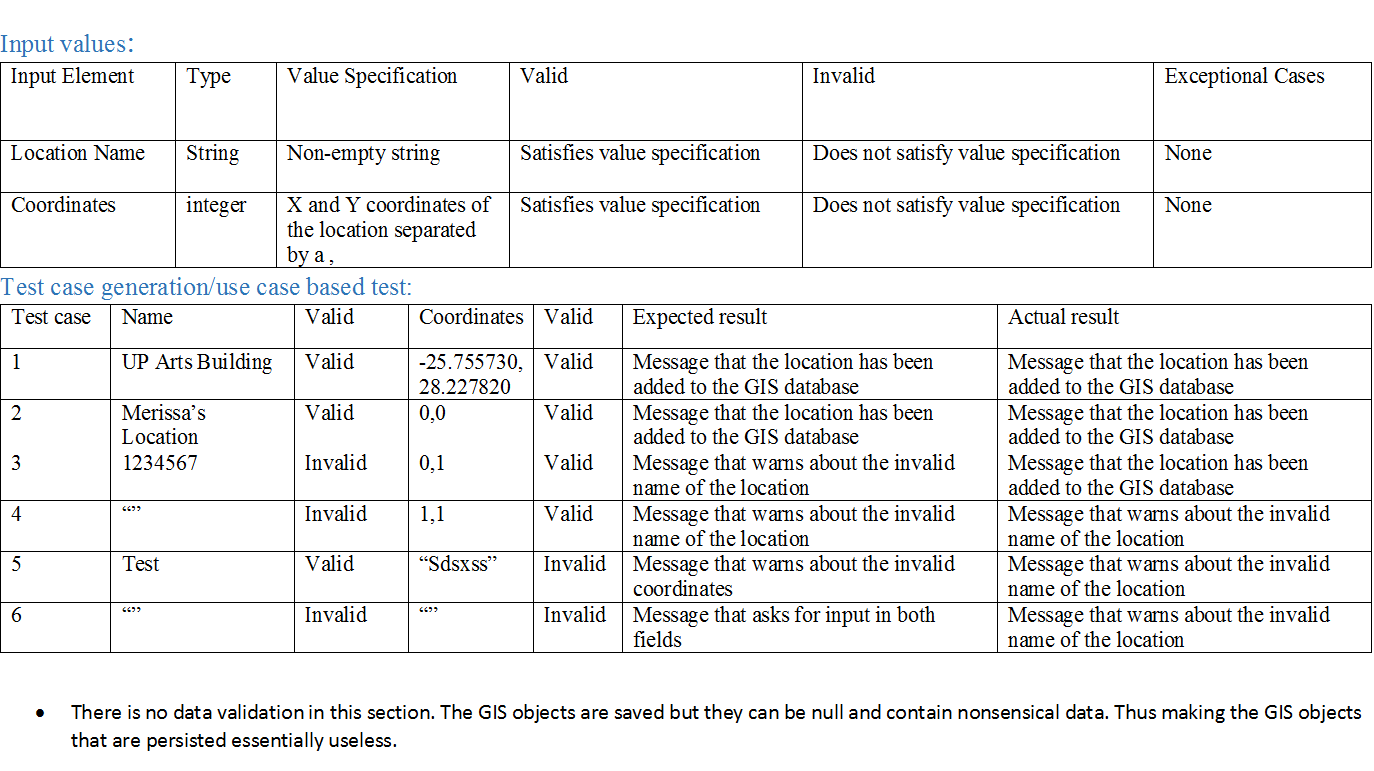
\includegraphics[width=180mm]{AddGISInformation.png}

\end{figure}


\subsection{Modify GIS information}



\begin{figure}[H]

    \label{tab:example}

\hspace*{-2.5cm} 

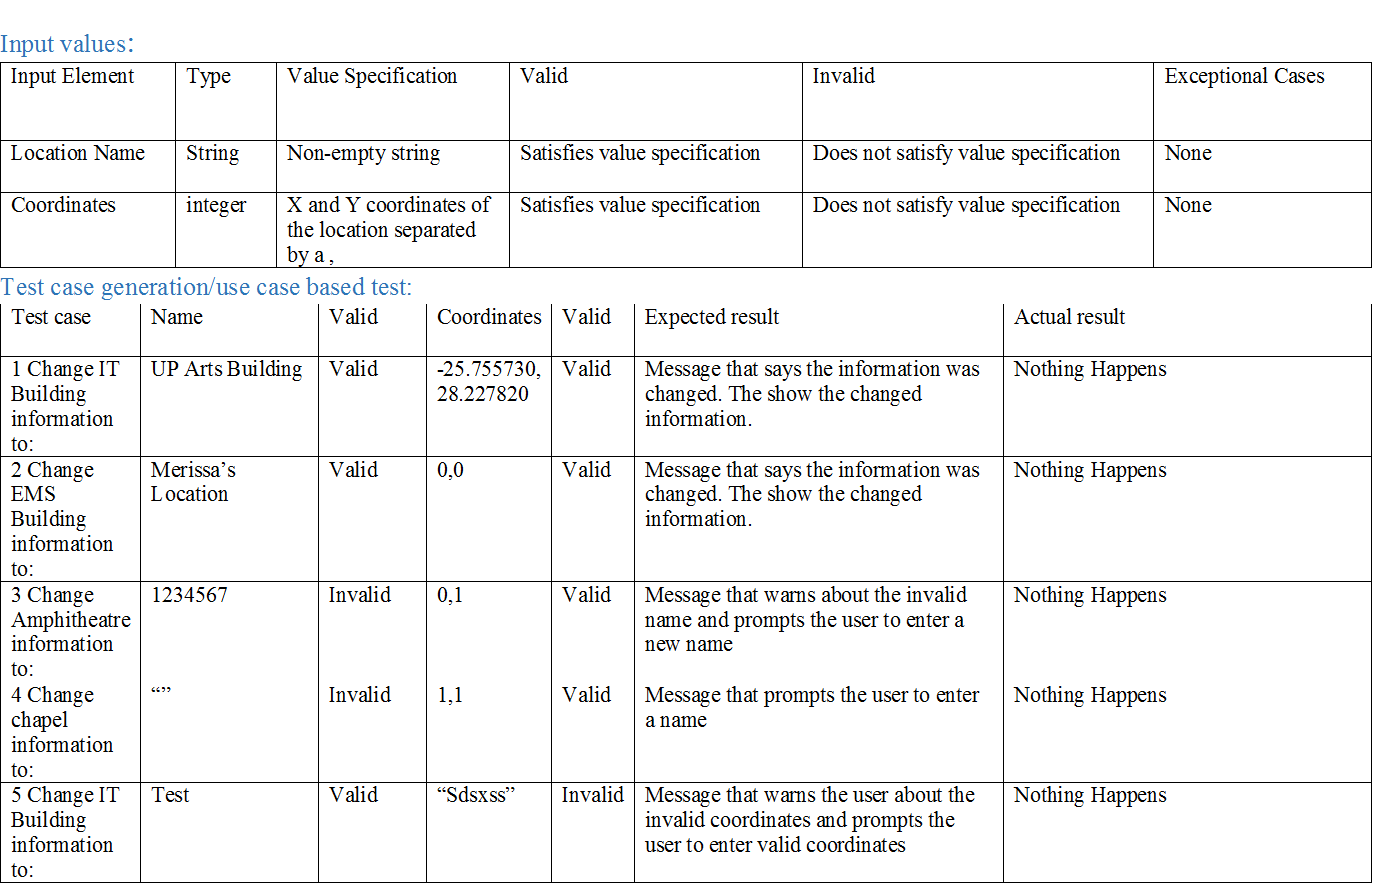
\includegraphics[width=180mm]{ModifyGISInformation.png}

\end{figure}




\subsection{Remove GIS information}

\begin{figure}[ht!]

\hspace*{-2.5cm} 

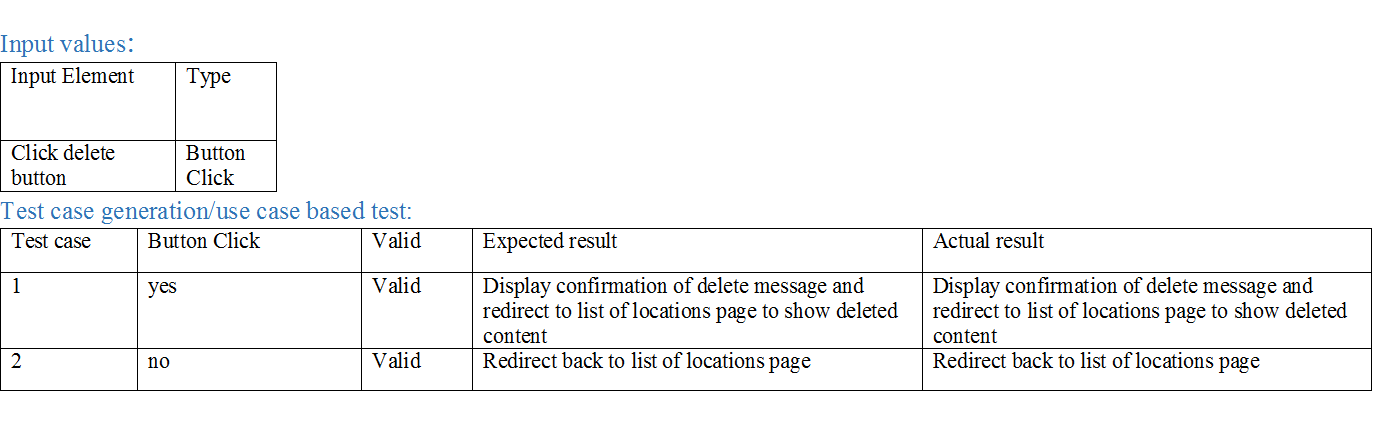
\includegraphics[width=180mm]{DeleteGISInformation.png}

\end{figure}


\subsection{Update GIS Map}

\begin{figure}[H]

\hspace*{-2.5cm} 

\includegraphics[width=180mm]{UpdateGISMap.png}

\end{figure}

\subsection{Modify GIS Map}

There is no functionality to modify the given map.


\section{Non-functional requirements}
\begin{figure}[H]

\hspace*{-2.5cm} 

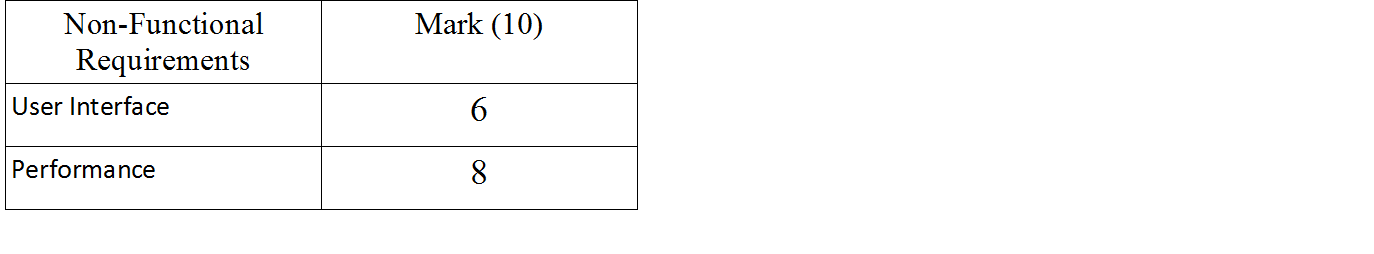
\includegraphics[width=180mm]{NFRMarks.png}

\end{figure}
\subsection{User interface}
•	The interface for adding GIS information is confusing. After saving the required information into the database, the information stays open and you cannot enter a new object until you refresh the page.
•	There is no limit on how far the user can zoom in and out. This leaves the user fully able to see the entire world map and view other locations, which should not be able to happen in the NavUp application.
•	The map can be dragged outside the boundaries of campus. This is not in the scope of the application.
•	The interface for GIS data modification is confusing. The labels do not guide the user in what he or she is doing in any way. 


\section{Points of interest}



\section{Navigation}
\end{document}